\documentclass[../../../../main.tex]{subfiles}
\begin{document}

\begin{flushright}
\footnotesize\textit{【自動文字起こし・要確認】}
\end{flushright}

\noindent
[\textbf{解}] $\angle AOB = \alpha, AP = x, BP = y$ とする ($r \ge l$). 又, $\angle PAB = \beta, \angle PBA = \delta$ とおく.

\bigskip

\noindent
\textbf{1° $P$ が劣弧 AB 上}

\begin{center}
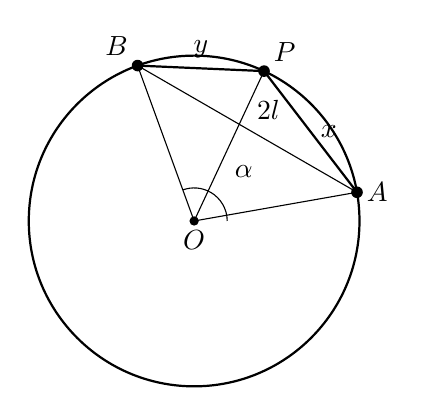
\begin{tikzpicture}[scale=1.4, >=stealth]
  \draw[thick] (0,0) circle (1.5);
  \fill (0,0) circle (1.2pt) node[below] {$O$};

  \coordinate (A) at (10:1.5);
  \coordinate (B) at (110:1.5);
  \coordinate (P) at (65:1.5);

  \fill (A) circle (1.5pt) node[right] {$A$};
  \fill (B) circle (1.5pt) node[above left] {$B$};
  \fill (P) circle (1.5pt) node[above right] {$P$};

  \draw (0,0) -- (A);
  \draw (0,0) -- (B);
  \draw (A) -- (B) node[midway, above right] {$2l$};

  \draw[thick] (P) -- (A) node[midway, right] {$x$};
  \draw[thick] (P) -- (B) node[midway, above] {$y$};

  \draw (0,0) -- (P);
  \draw (0.3,0) arc (0:110:0.3);
  \node at (0.45, 0.45) {$\alpha$};
\end{tikzpicture}
\end{center}

\noindent
$\triangle ABP$ に余弦定理を用いて
\[
4l^2 = x^2 + y^2 - 2xy \cos\left(\pi - \frac{\alpha}{2}\right) \quad \dots \text{①}
\]
又, 正弦定理を用いて
\[
\frac{2l}{\sin\left(\pi - \frac{\alpha}{2}\right)} = \frac{y}{\sin\beta} = \frac{x}{\sin\delta} = 2r \quad \dots \text{②}
\]
① に $xy = 2r\left(r - \sqrt{r^2 - l^2}\right)$ を代入,
\begin{align*}
(x+y)^2 &= 4l^2 - 2xy \cos\frac{\alpha}{2} + 2xy \\
&= 4l^2 + 4r\left(r - \sqrt{r^2 - l^2}\right)\left(1 - \cos\frac{\alpha}{2}\right) \quad \dots \text{③}
\end{align*}
又 ② と $0 < \frac{\alpha}{2} \le \frac{\pi}{2}$ から $\cos\frac{\alpha}{2} = \sqrt{1 - \left(\frac{l}{r}\right)^2}$ だから ③ に代入
\begin{align*}
(x+y)^2 &= 4l^2 + 4\left(r - \sqrt{r^2 - l^2}\right)^2 \\
&= 4\left[ l^2 + r^2 + r^2 - l^2 - 2r\sqrt{r^2 - l^2} \right] \\
&= 8\left(r^2 - r\sqrt{r^2 - l^2}\right)
\end{align*}
\[
x+y = \sqrt{8r\left(r - \sqrt{r^2 - l^2}\right)} \quad \dots \text{④}
\]
④ と題意から $t = r - \sqrt{r^2 - l^2}$ とおくと, $x, y$ は $P$ の2次式
\[
t^2 - 2\sqrt{2rt} + 2rt = 0
\]
の2解で
\[
x = y = \sqrt{2rt}
\]
より, $P$ は弧 AB の中点である.

\bigskip

\noindent
\textbf{2° $P$ が優弧 AB 上}

\begin{center}
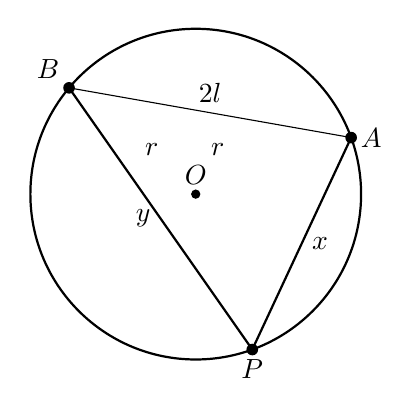
\begin{tikzpicture}[scale=1.4, >=stealth]
  \draw[thick] (0,0) circle (1.5);
  \fill (0,0) circle (1.2pt) node[above] {$O$};

  \coordinate (A) at (20:1.5);
  \coordinate (B) at (140:1.5);
  \coordinate (P) at (-70:1.5);

  \fill (A) circle (1.5pt) node[right] {$A$};
  \fill (B) circle (1.5pt) node[above left] {$B$};
  \fill (P) circle (1.5pt) node[below] {$P$};

  \draw (A) -- (B) node[midway, above] {$2l$};
  \draw[thick] (P) -- (A) node[midway, right] {$x$};
  \draw[thick] (P) -- (B) node[midway, left] {$y$};

  \node at (0.2, 0.4) {$r$};
  \node at (-0.4, 0.4) {$r$};
\end{tikzpicture}
\end{center}

\noindent
$\triangle ABP$ に正弦, 余弦定理を用いて
\begin{align*}
4l^2 &= x^2 + y^2 - 2xy \cos\frac{\alpha}{2} \quad \dots \text{①} \\
\frac{2l}{\sin\frac{\alpha}{2}} &= 2r \quad \dots \text{⑥}
\end{align*}
⑥ と $0 < \frac{\alpha}{2} \le \frac{\pi}{2}$ から $\cos\frac{\alpha}{2} = \sqrt{1 - \left(\frac{l}{r}\right)^2}$. だから ① に代入
\begin{align*}
(x+y)^2 &= 4l^2 + 2xy \cos\frac{\alpha}{2} + 2xy \\
&= 4l^2 + 4r\left(r - \sqrt{r^2 - l^2}\right)\left(1 + \sqrt{1 - \left(\frac{l}{r}\right)^2}\right) \\
&= 4l^2 + 4\left(r^2 - (r^2 - l^2)\right) \\
&= 8l^2
\end{align*}
\[
\therefore x + y = 2\sqrt{2}l
\]
従つて, $x, y$ は $P$ の2次式
\[
P^2 - 2\sqrt{2}l P + 2rt = 0
\]
の2解で
\[
P = \sqrt{2}l \pm \sqrt{2l^2 - 2r\left(r - \sqrt{r^2 - l^2}\right)}
\]
だから, A, B からの距離が各々 $\left( \sqrt{2}l \pm \sqrt{2l^2 - 2r\left(r - \sqrt{r^2 - l^2}\right)} \right)$ なる 2 点.
$P = A$ または $P = B$ の時は $AP \cdot BP = 0$ となるが, この時 $l = 0$ となり不適.

\bigskip

\noindent
以上 1°, 2° から, もとめるのは

劣弧 AB の中点, A, B からの距離が各々 $\left( \sqrt{2}l \pm \sqrt{2l^2 - 2r\left(r - \sqrt{r^2 - l^2}\right)} \right)$ なる優弧 AB 上の 2 点 (計 3 点) である. \hfill $\mathbin{/\mkern-5mu/}$

\newpage

\end{document}
